Steve va a convertir la mitad de su patio trasero en un gallinero. Su patio trasero es un rectángulo de 24 metros por 45 metros. Quiere poner una cerca de malla de gallinero que vaya de forma diagonal de una esquina a la opuesta.
\textbf{¿Cuántos metros de cerca va a necesitar Steve?}\\

\begin{solutionbox}{15cm}
    Sea $x$ la longitud diagonal de la cerca. Entonces el plano para el gallinero de Steve se ve así (ver Figura \ref{fig:proverb_pitagoras_09}):
    \begin{figure}[H]
        \centering
        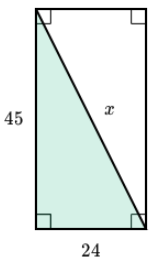
\includegraphics[width=0.2\linewidth]{../images/proverb_pitagoras_09.png}
        \caption{}
        \label{fig:proverb_pitagoras_09}
    \end{figure}
    Podemos usar el teorema de Pitágoras para obtener $x$.
    La ecuación del teorema de Pitágoras es:
    \[c^2=a^2+b^2\]
    donde $a$ y $b$ son las longitudes de los dos catetos del triángulo y $c$ es la longitud de la hipotenusa.
    En este caso, $a=24$, $b=45$ y $c=x$.
    \begin{align*}
        x^2 & =24^2+45^2    \\
        x^2 & =2,601        \\
        x   & =\sqrt{2,601} \\
        x   & =51
    \end{align*}
    Steve va a necesitar 51 metros de cerca.
\end{solutionbox}